\documentclass{beamer}

\usepackage{txfonts}
\usepackage{hyperref}
\usepackage{fancybox}
\usepackage{xfrac}
\usepackage{cancel}

\newcommand{\heart}{\ensuremath\heartsuit}

\usepackage{mathtools,amssymb}
\newcommand{\myarrow}{\scalebox{2}[2]{$\mathclap{\curvearrowleft}\mkern2.2mu
                                                 \mathclap{\curvearrowright}$}}

\DeclareMathOperator{\Bin}{\mathrm{Bin}}

\hypersetup{colorlinks=false,linkbordercolor=red,linkcolor=green,pdfborderstyle={/S/U/W 1}}

\addtobeamertemplate{navigation symbols}{}{ \hspace{1em}    \usebeamerfont{footline}%
    \insertframenumber / \inserttotalframenumber}

\geometry{papersize={15cm,12cm}}
\usepackage{lipsum}

\makeatletter
\newenvironment<>{contdproof}[1][\proofname]{%
    \par
    \def\insertproofname{#1\@addpunct{.}}%
    \usebeamertemplate{proof begin}#2}
  {\usebeamertemplate{proof end}}
\makeatother


\setbeamertemplate{theorems}[numbered]

\newtheorem*{nonumdefinition}{Definition}
\newtheorem*{nonumproblem}{Problem}
\newtheorem*{nonumtheorem}{Theorem}
\newtheorem*{nonumremark}{Remark}
\newtheorem*{answer}{Answer}
\newtheorem*{nonumremarks}{Remarks}
\newtheorem*{nonumexamples}{Examples}
\newtheorem*{nonumsolution}{Solution}
\newtheorem*{nonumexample}{Example}
\newtheorem*{nonumproposition}{Proposition}
\newtheorem{proposition}[theorem]{Proposition}


\usepackage{tikz}
\newcommand*\mycirc[1]{%
  \tikz[baseline=(C.base)]\node[draw,circle,inner sep=.7pt](C) {#1};\:
}

\newcommand\myheading[1]{%
  \par\bigskip
  {\color{blue}{\large #1}}\par\smallskip}

%\usetheme{Warsaw}
%\usetheme{Berkeley} %sample 1

\usetheme{Berlin} % sample 2
%\usetheme{AnnArbor} % sample 3

\let\otp\titlepage
\renewcommand{\titlepage}{\otp\addtocounter{framenumber}{-1}}

\title{Lecture 9 : Change of discrete random variable}
\author{}
\date{}

\begin{document}
\begin{frame}[plain]
\titlepage
\end{frame}

\begin{frame}
You have already seen (I hope) that whenever you have ``variables'' you need to consider \underline{change of variables}. Random variables are no different.

The notion of ``change of random variable'' is handle too briefly on page 103 of the text. \underline{This is something I will test you on.}

\begin{example}
Suppose $X\sim Bm\left(3,\dfrac{1}{2}\right)$.

\underline{line graph}

\medskip
\centerline{
\includegraphics{figure/fig1.eps}}
\smallskip

\underline{table}
\begin{equation*}
\begin{array}{|c|c|c|c|c|}
X & 0 & 1 & 2 & 3\\
\hline
P(X=x) & \dfrac{1}{8} & \dfrac{3}{8} & \dfrac{3}{8} & \dfrac{1}{8}\\
\hline
\end{array}\tag{b}
\end{equation*}
\end{example}
\end{frame}

\begin{frame}
Suppose what to define a new random variable $Y=2X-1$. 

How do we do it?

So how do we define $P(Y=k)$?

Answer - express $Y$ in terms of $X$ and compute so
\begin{align*}
P(Y=k) &= P(2X-1=k)\\[3pt]
       &= P\left(X=\dfrac{k+1}{2}\right)\tag{*}
\end{align*}
The right-hand site is the logical \underline{definition} of the left-hand side. 

But as is often the case in probability it is easier to pretend we know what $P(Y=k)$ means already and then the next two steps are a computation.
\end{frame}

\begin{frame}
So let's compute the $pmf$ of $Y$.

What are the possible values of $Y$?

From (*) $k$ is a possible value of $Y\Leftrightarrow \dfrac{k+1}{2}$ is a possible values of $X$.
$$
\Longleftrightarrow \ \dfrac{k+1}{2}=
\left\{
\begin{array}{c}
0\\
1\\
2\\
3
\end{array}
\right.
\quad \Longleftrightarrow \quad 
Y=
\left\{
\begin{array}{c}
-1\\
1\\
3\\
5
\end{array}
\right.
$$
Note

\centerline{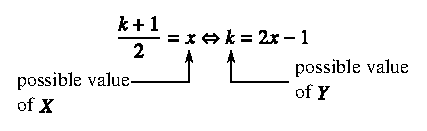
\includegraphics{figure/fig2.eps}}
\end{frame}

\begin{frame}
So the possible values of $Y$ are obtained by applying the function $h(x)=2x-1$ to the possible values of $X$. 

(note $Y=f(X)$).

\medskip
\centerline{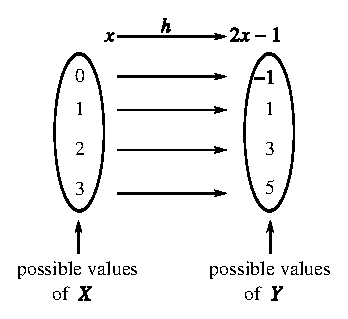
\includegraphics{figure/fig3.eps}}
\medskip

\underline{Just ``push forward'' the values of $X$.}
\end{frame}

\begin{frame}
\begin{nonumexample}[Cont.]
Now we have computed the possible values of $Y$ we need to compute their probabilities. Just repeat what we did
\begin{align*}
P(Y=-1) &= P(2X-1=-1)\\[3pt]
        &= P(X=0)=\frac{1}{8}\\[3pt]
P(Y=1) &= P(2X-1=1)\\[3pt]
       &= P(X=1)=\frac{3}{8}
\end{align*}
Similarly
$$
P(Y=3)=\frac{3}{8}\quad\text{and}\quad P(Y=5)=\frac{1}{8}
$$
\begin{center}
\begin{tabular}{|c|c|c|c|c|}
$X$ & $-1$ & $1$ & $3$ & $5$\\
\hline
$P(Y=y)$ & $\dfrac{1}{8}$ & $\dfrac{3}{8}$ & $\dfrac{3}{8}$ & $\dfrac{1}{8}$\\
\hline
\end{tabular}
\end{center}
\end{nonumexample}
\end{frame}

\begin{frame}
So we have the ``same probabilities'' as before namely $\dfrac{1}{8}$, $\dfrac{3}{8}$, $\dfrac{3}{8}$, $\dfrac{1}{8}$ it is just then are pushed-forward to new locations

\medskip
\centerline{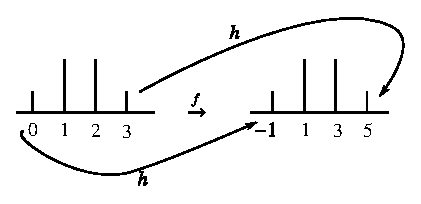
\includegraphics{figure/fig4.eps}}
\end{frame}

\begin{frame}

\end{frame}

\begin{frame}

\end{frame}

\begin{frame}

\end{frame}

\begin{frame}

\end{frame}

\begin{frame}

\end{frame}

\begin{frame}

\end{frame}


\end{document}


